\chapter{Dataset}
\label{chap:math}

We first had to find a suitable dataset to evaluate the scientific question.
Thus we consulted literature and the internet to find a dataset that would suit our needs.
We needed a news dataset that would suffice these requirements:

\begin{itemize}
    \item Contains content of the article for each sample
    \item Partially contains category, authors, publication date, publication server
    \item Size of at least 200k samples
    \item Language: Czech
\end{itemize}


The closes to our requirements we found were:
\begin{itemize}
    \item \cite{strakaSumeCzechLargeCzech2018a} - 1M czech news articles.

          While sufficiently large and in the correct language,
          it doesn't contain neither category, not author metadata.
          However, the paper provides valuable information about dataset extraction
          and cleaning of the dataset.
    \item \cite{misraNewsCategoryDataset2022} - 210k english news articles.

          While it contains both category and author metadata,
          the language is English, and the dataset doesn't have the content of the articles.
\end{itemize}

As neither dataset suited our needs, we created our own dataset.


\section{Dataset creation}
\label{sec:dataset-creation}

\subsection{Data source}
We initially decided to collect the data from these news servers:
\begin{itemize}
    \item Seznamzpravy.cz
    \item Irozhlas.cz
    \item Novinky.cz
    \item Aktuálně.cz
    \item Idnes.cz
    \item Ihned.cz
    \item Deník.cz
\end{itemize}

These sources were chosen due to their popularity and high amount of articles.
To get articles, we had two options:
\begin{enumerate}
    \item Use a web spider to crawl the live website.
    \item Use a web archive that contains crawled articles.
\end{enumerate}
We chose the second option because crawling live websites is tricky,
as the servers would be too fast to block the crawler due to too many requests. Another advantage of the second approach is that we would probably not be able to get as many articles as
with web crawler since there might be no links to old articles anymore.

\subsection{Webarchive}
As a web archive, we chose a CommonCrawl~\cite{CommonCrawl}.
CommonCrawl is an open-source project crawling the web and storing the data.
The data are stored as a WARC\todo{Should I somehow cite this ?} files in Amazon's S3 storage.
The data can then be queried using Amazon's big data tools or CommonsCrawl's API.
The data stored in the archive have been collected since 2008 with various frequencies,
but since 2014 they have been collected monthly.

\subsection{Data extraction}
\subsubsection{CC Extractor}
To extract the data, we built a program that can extract the data from a CommonCrawl
based on the URL, data, etc\dots. The program was
created strongly emphasizing scalability and realability\todo{I Guess I should explain these terms?}.
It's separated into two parts:
\begin{enumerate}
    \item Aggregator -
          Extracts links from CommonCrawl API for specified URLs and sends them to a Processor.
    \item Processor -
          Loads the WARC data from S3 and extracts the requested metadata.
          For extraction, we used python's beautifulsoup library.
\end{enumerate}
Both of them can be scaled based on the needs.
The connection between the Aggregator and processor can be made using various middlewares.
As of now, the used middleware is ActiveMQ Aremis~\cite{ActiveMQ}.
When the Aggregators send links to Processors,
they are filtered based on the normalized version(URL without query, duplicated '/' etc\dots).
\todo{Should I go more in-depth with the description ?}
\subsubsection{Extraction}
We have done extraction on 12.12.2022.
We set the extractors to only output articles in which the processor successfully
extracted the content and headline.
We set the aggregators to process crawls from 1.1.2008 to 31.8.2022.
We used the~\cite{UFALAIC} for the deployment of the extractor.
We run one aggregator and four processors for each server,
totaling seven extractors and 28 processors.
As for orchestration, while the program has working docker support,
the cluster doesn't support it, and thus we used shell scripts for deployment.
The 49M URLs were processed, of which the processor received 82M
and successfully processed 31M articles.

Once we extracted the data, we started with filtering and postprocessing.
\subsection{Filtering}

Filtering was done in several steps. The filtering was done with hugging face datasets library as it allows for distributed processing of the data.
This allowed us to filter the data in a few hours on a single machine.



\subsection{Ihned.cz articles}
Similar to~\cite{strakaSumeCzechLargeCzech2018a}, we found that the Ihned.cz articles contained
a high number of paywalled articles and overall didn't contain many samples.
We thus decided to drop it.

\subsection{CZ filtering}
Since we were interested in Czech articles, we decided to filter out articles
not in the Czech language. For this purpose,
we used FastText Language detection model~\cite{joulinFastTextZipCompressing2016,joulinBagTricksEfficient2016}. The model was run on each line article of content which. This allowed us to interpret fraction of lines that were predicted as czech as confidence of article being czech.
We inspected the articles with lower confidence, and the most occurring problems were:
\begin{enumerate}
    \item Articles in Ukraine language on Seznamzpravy.cz, due to the recent war in Ukraine
    \item Articles with a list of sports results where most texts were
          the result, team, and match highlights.
    \item Articles with comparison tables, e.g., mobile comparison
    \item Galeries, there were few articles with galleries of pictures or videos with little text.
    \item English articles on Idnes.cz and Irozhlas.cz
\end{enumerate}
Since we had many articles, we decided to filter out articles with a confidence lower than 1.0.

\subsubsection{Filtering by Article Statistics}
\label{sec:filtering-by-article-statistics}
The main goal of this step was to filter out either wrongly parsed
or non-news articles(plain sports results, weather, tables, videos/photos\dots).
We thus inspected article content based on several properties
and set the following thresholds to remove unwanted characters:
\begin{enumerate}
    \item General:
          \begin{enumerate}
              \item Content length - $(400, \inf)$
              \item Headline length - $(20, \inf)$
              \item Brief length - $(40, \inf)$
              \item Publication date - $(1.1.2000, 31.8.2022)$
          \end{enumerate}
    \item Content:
          \begin{enumerate}
              \item Average word length - $(4.0, \inf)$
              \item Num of words / Lenght - $(0.11, 0.22)$
              \item Non-alphanumeric characters / Length - $(0, 0.045)$
          \end{enumerate}
\end{enumerate}

During the inspection, we further found the following problems:
\begin{enumerate}
    \item Headline cuts

          When observing articles with short headlines, we found that the headlines
          were cut in the middle of words.
          It was because the extractor had a function that would remove anything after `-'.
          In headlines, it was supposed to prevent the bloat like `- Aktuálně.cz'. However,
          we didn't anticipate this would also remove words like start-up, etc\dots.
          We removed this rule and reran the whole extraction.
    \item Article character length

          When observing article length at Novinky.cz and Seznamzpravy.cz,
          we found many articles with sizes of less than 100 characters.
          We found that this was due to an extraction error.
          For these two sites, we were extracting content by CSS classes.
          However, we didn't include all possible classes as they are likely autogenrated;
          thus, sometimes extractor extracted only headers.
          We tried to fix the problems by adding more classes and generalizing the CSS selectors,
          reducing the issue but not eradicating it. We thus decided to resolve this problem
          by the content length rule.

    \item Brief/Headline length drops

          When inspecting Aktualne.cz we found that headlines
          had steep drops in several samples at specific headline lengths (55, 60, 85).
          However, we haven't found any problems with such headlines.
          We assume these inconveniences result from internal rules for writers at Aktualne.cz.
\end{enumerate}

\subsubsection{Filtering by headline content}
As in \cite{strakaSumeCzechLargeCzech2018a}, many articles
contained prefixes at headlines like 'VIDEO: ', 'FOTO: ', 'GALERIE: ' etc\dots.
Since we were interested in the articles and not galleries,
we dropped the articles with prefixes that indicate not a non-article.
However, unlike \cite{strakaSumeCzechLargeCzech2018a}, we haven't removed these prefixes
in non-filtered headlines/briefs.




\subsubsection{Headline/Brief/Content dedupliation}
The last filtering round removed articles with identical briefs, headlines, or content.

We were afraid that this would also affect the article across different servers.
It turned out that the deduplication only deleted around 3K articles
because of cross-server duplicates.

When choosing which duplicate to use, we took the one with the most metadata filled
or the longer article length.

Therefore, every Brief/Content/Headline is unique in the dataset.

\subsection{Data Augmentation and Postprocessing}

\subsubsection{Category}
\label{sec:category}
Due to the wide variety of collected data, we had to normalize categories.
After extraction, we got a total of 3383 categories.
Since there was considerable overlap between each category,
we selected 25 categories among the most popular ones.
We focused on choosing the categories with the most samples
while ensuring a small overlap between selected categories.
That's why we dropped categories like Zprávy, Tipy, Vaše zprávy, Ostatní, etc\dots,
even though they had a high amount of samples.


We then mapped from the remaining categories to these 25 categories if such a mapping was possible.
Examples of such mappings are:
\begin{enumerate}
    \item Football, Tennis, Biatholon\dots $\rightarrow$ Sport
    \item Praha, Domažlicko, Ústecko\dots $\rightarrow$ Domácí
    \item Ona, Ženy, Móda\dots $\rightarrow$ Životní styl
\end{enumerate}


\subsubsection{Authors}
\label{sec:authors}
After extraction, there were 27K unique authors.
The obvious problem was that not all authors were people.
Surprisingly, the most prevalent were the news institutions: ČTK, IDnes, MF DNES, etc\dots.
There were also many nicknames we couldn't decode, companies,
and common names like Redakce, externí, etc\dots.

We thus employed heuristics and manual filtering
to mitigate these problems and ended up with 11K authors.
As for postprocessing, we removed occupation, academic titles, and mysterious form names.

\subsubsection{Gender and cumulative gender}
\label{sec:gender}
As gender was not provided in articles, we had to guess it from names.
There are numerous ways to do it; the simplest would be to categorize all names ending with 'á' as WOMAN and MAN otherwise.
However, we decided to use a model for the preiction.
As \cite{seboPerformanceGenderDetection} suggests,
the \cite{NamsorNameChecker} offers great accuracy with a reasonable amount of unrecognized names.
We thus used it for the prediction.

For cumulative gender, we used the following rules:
\begin{enumerate}
    \item If all authors of the article are MAN $\rightarrow$ MAN
    \item If all authors of the article are WOMAN $\rightarrow$ WOMAN
    \item MIXED otherwise
\end{enumerate}

\subsubsection{Content, Brief, Headline Postprocessing}
We used the following postprocessing steps for content, brief, and headline:
\begin{enumerate}
    \item Replace '\textbackslash{n}','\textbackslash{r}','\textbackslash{t}' with spaces
    \item Truncate spaces
    \item Convert named and numeric character references to Unicode
    \item Normalize Unicode characters to their base combined form
\end{enumerate}
As for Brief and Headline, we capitalized the first letter
and added a dot at the end if there wasn't one.

\subsection{Splits}
Since we were interested in predicting the future,
we decided to split the data into train, validation, and test set based on the publication date.

The sets are, therefore, not random but ordered by publication date. Train set having the earliest, while test the latest.
If the sample didn't have a publication date, we randomly assigned it to one of the sets.
The ratio between the sets was selected to $85:7.5:7.5$.
\section{Dataset summary}
\begin{table}[h]
    \centering\footnotesize\sf
    \begin{tabular}{lrrrrr}
        \toprule
        {}              & Size    & Unique Authors & Categories & Date Range            & Article words \\
        \midrule
        Denik.cz        & 664133  & 2497           & 18         & 27.3.2007 - 6.8.2022  & 332           \\
        Novinky.cz      & 321417  & 2518           & 17         & 20.12.2002 - 6.8.2022 & 274           \\
        Idnes.cz        & 295840  & 4385           & 21         & 3.1.2000 - 9.8.2022   & 423           \\
        Irozhlas.cz     & 167588  & 1900           & 8          & 8.7.2000 - 25.6.2022  & 287           \\
        Aktualne.cz     & 112960  & 633            & 19         & 26.10.2005 - 6.8.2022 & 468           \\
        Seznamzpravy.cz & 65472   & 382            & 11         & 14.9.2016 - 6.8.2022  & 443           \\
        \midrule
        Total           & 1627410 & 10930          & 25         & 3.1.2000 - 9.8.2022   & 362           \\
        \bottomrule
    \end{tabular}
    \caption{Table representing the dataset summary. Article words were calculated based on Moses tokenization.}
    \label{tab:dataset_summary}
\end{table}
The summarization of the dataset is shown in \autoref{tab:dataset_summary}.
Since we are interested in the classification of the author's gender, category,
article's server and publication day of the week, we provide a more detailed summary of these properties,

\subsection{Category}
\begin{table}[h]
    \centering\footnotesize\sf
    \begin{tabular}{lrrr}
        \toprule
        {}           & Train  & Validation & Test  \\
        \midrule
        Domácí       & 216889 & 26326      & 31195 \\
        Sport        & 154743 & 18565      & 18134 \\
        Zahraniční   & 147426 & 8344       & 9705  \\
        Kultura      & 78330  & 2838       & 3084  \\
        Ekonomika    & 70506  & 3847       & 2761  \\
        Krimi        & 53711  & 644        & 1236  \\
        Technologie  & 29337  & 1952       & 1763  \\
        Koktejl      & 23900  & 295        & 161   \\
        Životní styl & 23129  & 1839       & 1500  \\
        Auto         & 14924  & 1356       & 1198  \\
        \midrule
        Other        & 66124  & 12078      & 11615 \\
        \midrule
        Total        & 879019 & 78084      & 82352 \\
        \bottomrule
    \end{tabular}
    \caption{Table representing top 10 categories distribution per dataset. Other category contains all the remaining categories.}
    \label{tab:category}
\end{table}
\begin{figure}[h]
    \centering
    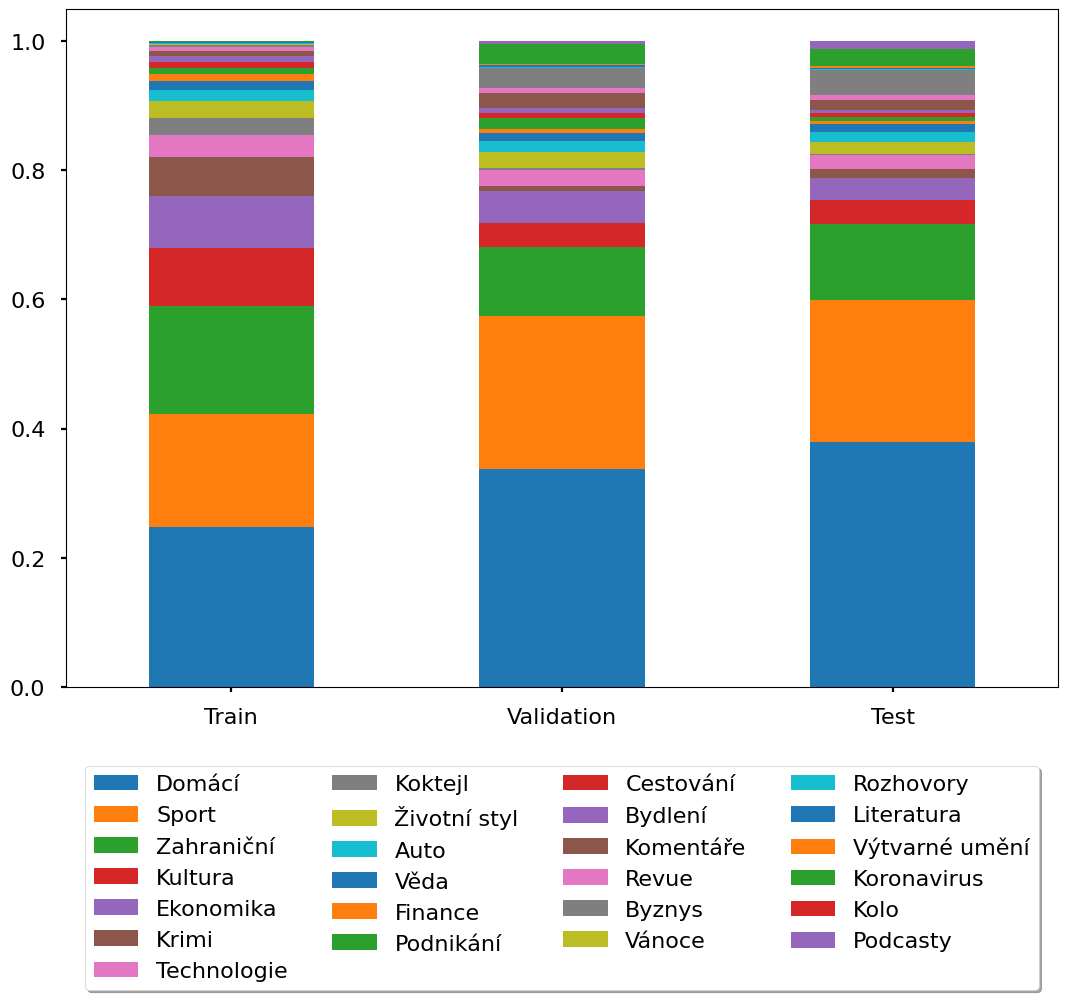
\includegraphics[width=.6\linewidth]{img/tasks_graph/category.png}
    \caption{Graph depicting proportion of article\'s category among the datasets}
    \label{fig:category_graph}
\end{figure}
As seen in \autoref{tab:category},\autoref{fig:category_graph}, the most frequent category is Domácí.
We know it might overlap with other categories like Ekonomika, but we decided to keep it separate.
All the categories but 'Kolo' are represented in each split. The 'Kolo' is missing in the validation split.

\subsection{Server}
\begin{table}[h]
    \centering\footnotesize\sf
    \begin{tabular}{lrrr}
        \toprule
        {}           & Train   & Validation & Test   \\
        \midrule
        Denik        & 553799  & 53980      & 56354  \\
        Novinky      & 313274  & 5647       & 2496   \\
        Idnes        & 246441  & 27673      & 21726  \\
        Irozhlas     & 148388  & 10530      & 8670   \\
        Aktualne     & 93281   & 10037      & 9642   \\
        Seznamzpravy & 28115   & 14189      & 23168  \\
        \midrule
        Total        & 1383298 & 122056     & 122056 \\
        \bottomrule
    \end{tabular}
    \caption{Table representing server distribution per dataset.}
    \label{tab:server}
\end{table}
\begin{figure}[h]
    \centering
    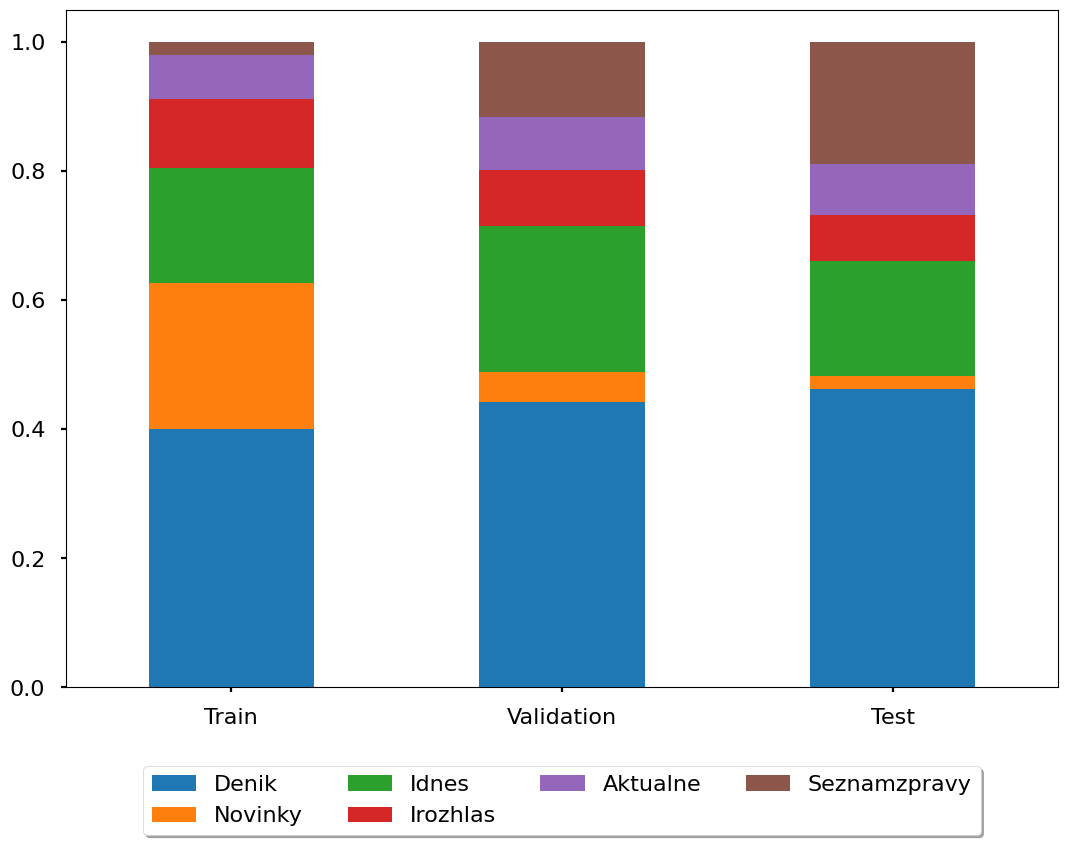
\includegraphics[width=.6\linewidth]{img/tasks_graph/server.png}
    \caption{Graph depicting proportion of news servers among the datasets}
    \label{fig:server_graph}
\end{figure}
From \autoref{tab:server} and \autoref{fig:server_graph} we can see that the most frequent server is Deník.cz.
That is due to regional coverage,
which is not present on the other servers. We can also see
There is a shallow representation of the Seznamzprávy in the training set.
This is because the server was launched the latest, among others, in 2016.
The extinction of Novinky.cz is likely explained by \autoref{sec:filtering-by-article-statistics}.


\subsection{Publication Day of the Week}
\begin{table}[h]
    \centering\footnotesize\sf
    \begin{tabular}{lrrr}
        \toprule
        {}        & Train   & Validation & Test   \\
        \midrule
        Monday    & 216382  & 18746      & 18891  \\
        Tuesday   & 231714  & 20359      & 19968  \\
        Wednesday & 235415  & 20076      & 20479  \\
        Thursday  & 232115  & 19983      & 20547  \\
        Friday    & 221029  & 19194      & 18837  \\
        Saturday  & 131289  & 12487      & 12148  \\
        Sunday    & 115354  & 11211      & 11186  \\
        \midrule
        Total     & 1383298 & 122056     & 122056 \\
        \bottomrule
    \end{tabular}
    \caption{Table representing day of week distribution per dataset.}
    \label{tab:day_of_week}
\end{table}
\begin{figure}[h]
    \centering
    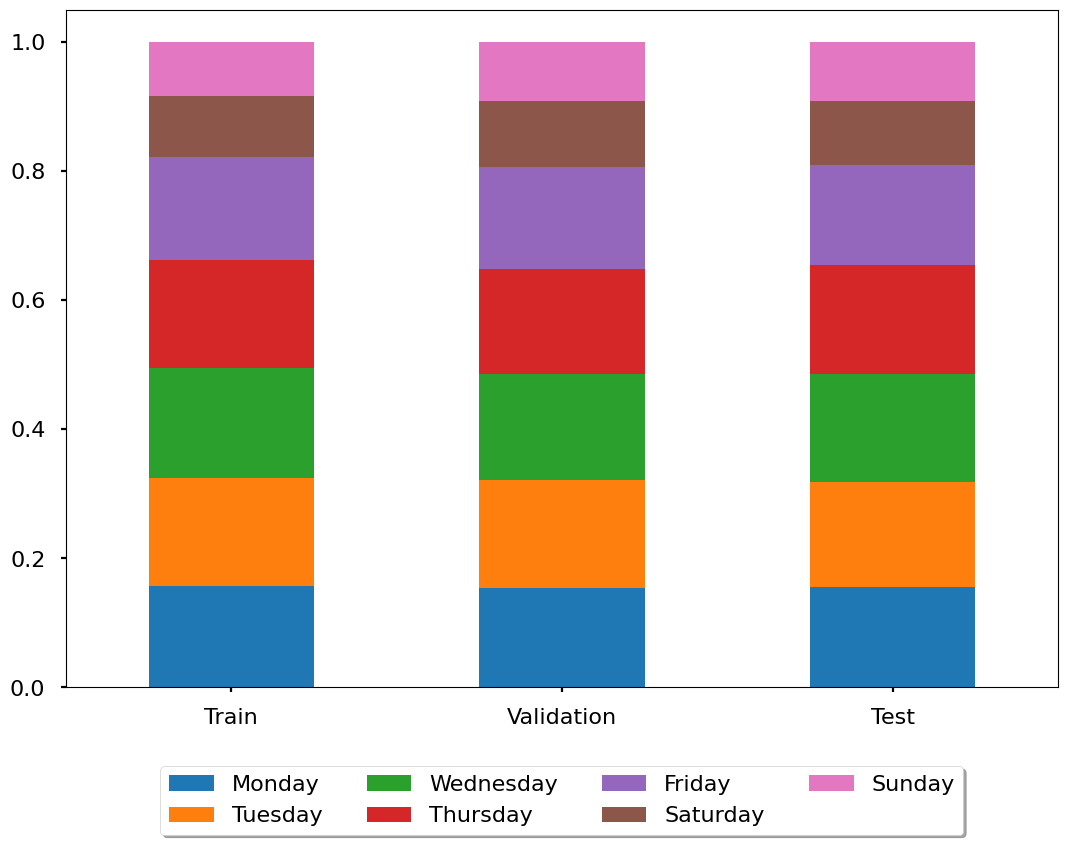
\includegraphics[width=.6\linewidth]{img/tasks_graph/day_of_week.png}
    \caption{Graph depicting proportion of weekdays among the datasets}
    \label{fig:day_graph}
\end{figure}
The days of the week are evenly distributed among the datasets, as seen in \autoref{tab:day_of_week} and \autoref{fig:day_graph}.
We can see that there is a bit more articles published on weekdays than on weekends.

\subsection{Author's gender}
\begin{table}[h]
    \centering\footnotesize\sf
    \begin{tabular}{lrrr}
        \toprule
        {}    & Train  & Validation & Test  \\
        \midrule
        Man   & 566270 & 52621      & 52675 \\
        Woman & 312109 & 28829      & 28997 \\
        Mixed & 41461  & 1486       & 1597  \\
        \midrule
        Total & 919840 & 82936      & 83269 \\
        \bottomrule
    \end{tabular}
    \caption{Table representing Gender distribution per dataset.}
    \label{tab:gender}
\end{table}
\begin{figure}[h]
    \centering
    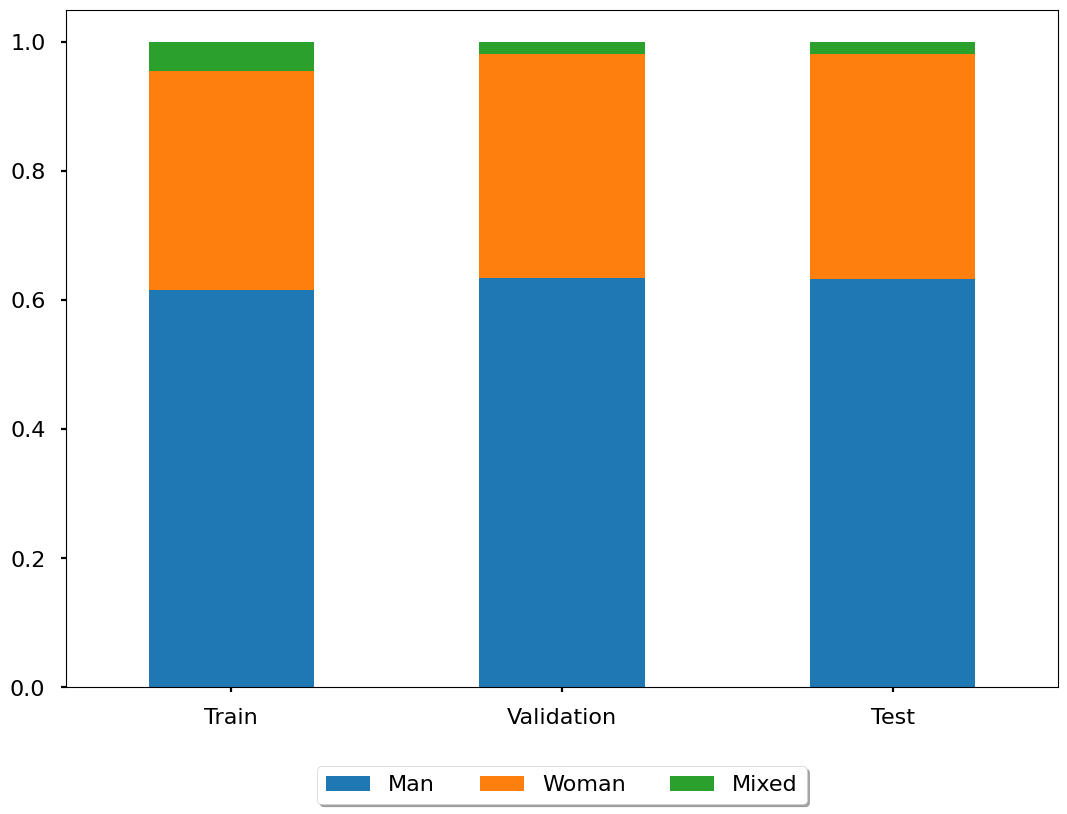
\includegraphics[width=.6\linewidth]{img/tasks_graph/authors_cum_gender.png}
    \caption{Graph depicting proportion of authors\'s gender among the datasets}
    \label{fig:gender_graph}
\end{figure}
We were a bit surprised by the fact that the authors are primarily men (around $60\%$) as seen in \autoref{fig:gender_graph}, \autoref{tab:gender}.
It might be due to \autoref{sec:gender} mostly missclassfing female authors as male, or there might be a bias in the Czech media. 
